\section{Simulations and labels}
\label{sec:sims}

\subsection{TNG-Cluster}
\begin{itemize}
  \item 352 zoom clusters, $M_{500} \sim 10^{14.0-15.3}\,{\rm M_\odot}$,
        snapshot 99 ($z = 0$); three orthogonal projections each.
  \item Plus the same clusters at the full snapshot 91 ($z = 0.0994$,
        1.3\,Gyr earlier; 351 matched): 0.03\,dex lighter, and a merger time
        that correlates only weakly with the same cluster's at $z = 0$
        (Spearman 0.32), so mostly new examples rather than near-duplicates.
        Each snapshot uses its own FOF centre, \rfive\ and \mfive; both
        epochs of a cluster are always in the same cross-validation fold.
  \item Halo-centred on \texttt{GroupPos}; note the earlier weight-centroid
        centring was off by a median 0.70\,\rfive\ (Appendix~\ref{app:audit}).
\end{itemize}

\subsection{Radio emission model}
\begin{itemize}
  \item Hoeft \& Br\"uggen (2007) DSA emission per shocked cell
        (Mach $>1.3$, positive energy dissipation), as in Lee et al.\ (2024).
  \item Key finding: the emission is pathologically concentrated (one cell
        carries a median 29.5\% of a cluster's radio weight), and the cells
        that dominate are cold ($\sim$66\,000\,K), 379$\times$ overdense,
        Mach $\sim$26 gas at 1.37\,\rfive\ -- not diffuse ICM. Its origin is not traced:
        cold, dense gas such as stripped satellite ISM is a consistent
        interpretation, not a demonstrated one (review F9).
  \item Density cut $n_{\rm H} < 10^{-4}\,{\rm cm^{-3}}$ on shock cells:
        motivated by the DSA model's own assumption of ICM shocks, and it
        improves realism against LoTSS. It gives no demonstrated accuracy
        gain on the clean maps under the current protocol (no cut 0.500, cut
        0.485; paired seeds $p = 0.16$); the earlier $p = 0.010$ gain came
        from the old checkpoint selection and does not survive.
  \item Emission at 144\,MHz: the $(\nu/1.4\,{\rm GHz})^{-s/2}$ factor
        depends on each cell's Mach number, so it is applied per cell, not
        as one rescaling. With the density cut it changes little: cluster
        fluxes move by 0.035\,dex (s.d.), 5\% of each map's flux moves
        between pixels, CNN $R^2$ $0.487 \to 0.485$ (paired, 5 seeds). All
        results in this paper are at 144\,MHz unless marked otherwise.
  \item Snapshot redshift enters through comoving-to-physical units and
        $B_{\rm CMB} \propto (1+z)^2$.
  \item Images: arcsinh-stretched projected weight, 128\,px over
        $\pm4$\,\rfive.
\end{itemize}
\begin{figure*}
  \centering
  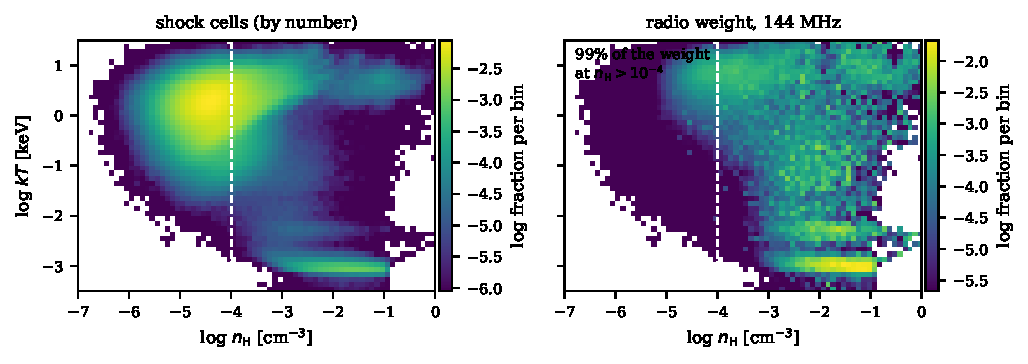
\includegraphics[width=\textwidth]{fig_phase.pdf}
  \caption{Where the radio weight sits. Density--temperature distribution
  of all shock cells (Mach $>1.3$) in the 352 snapshot-99 clusters, each
  cluster normalised to unit total, by number (left) and by 144\,MHz radio
  weight without any cut (right). Most shocks are in the diffuse ICM
  ($n_{\rm H} \sim 10^{-5}$--$10^{-4}$\,cm$^{-3}$, $kT \sim 1$\,keV), but
  a median 99 per cent of the weight (16--84 per cent: 96--100) is in cells
  denser than $10^{-4}$\,cm$^{-3}$, much of it cold
  ($kT \sim 10^{-3}$\,keV), strongly shocked gas (origin not traced; stripped satellite gas is one
  consistent interpretation). The dashed line
  is the cut we apply: it lowers the brightest cell's share of a cluster's
  emission from 25 to 5 per cent and the weight-averaged Mach number from
  62 to 4.8.}
  \label{fig:phase}
\end{figure*}

\subsection{X-ray mocks}
\begin{itemize}
  \item pyxsim APEC emission from hot, non-star-forming gas; soxs
        Chandra ACIS-I (Cycle 22) response, PSF, dither, particle
        background; 2\,Ms, observed at $z = 0.05$ (snapshot 99) and at
        $z = 0.0994$ (snapshot 91). The snapshot-91 images are moved onto
        the snapshot-99 physical grid, splitting each pixel's counts
        binomially between the blocks it overlaps.
  \item Field of view: only the ACIS-I square has data, $\pm$500\,kpc
        (0.3--0.6\,\rfive), \emph{not} $\pm1\,r_{500}$.
  \item Stretch: bare arcsinh is the identity at X-ray count rates; we use
        ${\rm arcsinh}(x/a)$ with one global $a$ (Section~\ref{sec:xray}).
\end{itemize}

\subsection{Merger-time labels}
\begin{itemize}
  \item Time since the most recent collision of \emph{any} mass ratio
        (merger catalogue of Lee et al.\ 2024; median ratio 1:11).
  \item Pseudo-TSC (interpolated merger-score crossing) agrees at
        Spearman 0.961; which one we headline, and why.
  \item At earlier snapshots the past-only merger score is required: the
        default score also counts mergers still to come, and differs for
        42\% of halos at snapshot 91.
  \item Major-merger-only labels are far less predictable
        ($R^2$ 0.435 $\to$ 0.074, old protocol: best epoch chosen on the
        evaluation fold, review F7; rerun or drop): radio morphology reflects recent
        disturbance of any size.
\end{itemize}
\begin{figure*}
  \centering
  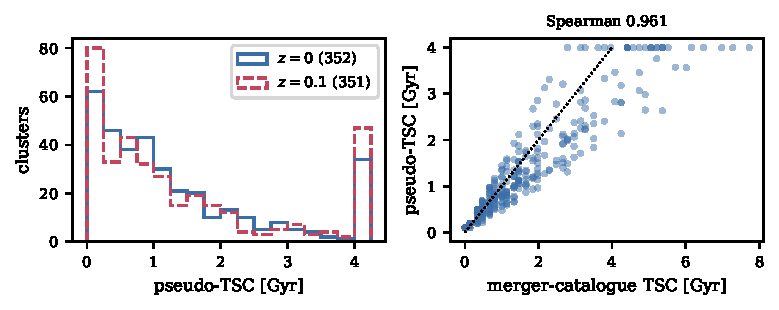
\includegraphics[width=0.75\textwidth]{fig_labels.pdf}
  \caption{The regression target. Left: pseudo-TSC at $z = 0$ (snapshot 99)
  and $z = 0.1$ (snapshot 91); medians 0.92 and 0.91\,Gyr, with 10 and
  13 per cent of clusters at the 4\,Gyr cap (merger score never crosses
  0.5 within the window). Right: pseudo-TSC against the merger-catalogue
  time since collision at $z = 0$ (346 clusters with a recorded collision;
  Spearman 0.961); the catalogue clock runs past the cap.}
  \label{fig:labels}
\end{figure*}
